\documentclass[
    12pt,
    a4paper,
    oneside
]{article}

% -------------------------------------------------
% PACOTES
% -------------------------------------------------

\usepackage[brazil]{babel}
\usepackage[utf8]{inputenc}
\usepackage[T1]{fontenc}

\usepackage{times}
\usepackage{indentfirst}
\usepackage{graphicx}
\usepackage{float}
\usepackage{xcolor}
\usepackage{amsmath}
\usepackage{setspace}
\usepackage{geometry}
\usepackage{titlesec}
\usepackage{caption}

% -------------------------------------------------
% CONFIGURAÇÕES ABNT
% -------------------------------------------------

\geometry{
    a4paper,
    left=3cm,
    right=2cm,
    top=3cm,
    bottom=2cm
}

\setlength{\parindent}{1.25cm}
\setlength{\parskip}{0cm}

\onehalfspacing

% -------------------------------------------------
% INÍCIO DO DOCUMENTO
% -------------------------------------------------

\begin{document}

% -------------------------------------------------
% CAPA
% -------------------------------------------------

\begin{titlepage}

    \begin{minipage}[c]{0.3\textwidth}
        \raggedright
        \raisebox{0pt}[\height][0pt]{%
            
\includegraphics[width=4cm]{imagens/Logo_UnB.png}%
        }
    \end{minipage}
    \hfill
    \begin{minipage}[c]{0.7\textwidth}
        \centering
        \textbf{\LARGE Universidade de Brasília}\\[0.25cm]
        \textbf{\large Departamento de Ciência da Computação}\\[0.1cm]
    \end{minipage}

    \begin{center}
        \vspace{4cm}

        {\Large \textbf{Teleinformática e Redes 2}}

        \vspace{1cm}

        {\large Tarefa Camada de Transporte}

        \vfill

        \textbf{Membros}

        \vspace{0.5cm}

        Daniel Lincoln Lopes de Souza -- 202042829\\
        Isabela Soares Furlan -- 231013636\\
        Luiz Fernando Candido Soaris -- 190092025

        \vfill

        Brasília -- DF\\
        \today

    \end{center}

\end{titlepage}

% -------------------------------------------------
% SUMÁRIO
% -------------------------------------------------

\tableofcontents
\newpage

% -------------------------------------------------
% INTRODUÇÃO
% -------------------------------------------------

\section{Introdução}

Este relatório apresenta a análise de uma conexão TCP utilizando o Wireshark, com foco em mecanismos da camada de transporte. A partir da captura de tráfego e das ferramentas de análise disponíveis, foram investigados aspectos relacionados ao estabelecimento da conexão, transferência de dados, controle de congestionamento, retransmissões e desempenho da comunicação.

Os resultados obtidos permitiram observar o comportamento do protocolo TCP em uma sessão real e relacionar as evidências experimentais aos conceitos estudados na disciplina.

\section{Questões objetivas}

\subsection{Questão 1}
O estabelecimento da conexão TCP foi identificado por meio do three-way handshake, composto pelos pacotes SYN, SYN-ACK e ACK observados no início do fluxo TCP analisado.

\subsubsection*{(a) RTT entre o SYN e o SYN-ACK}

O valor do RTT foi obtido diretamente do campo \textit{Time since previous frame in this TCP stream} presente no pacote SYN-ACK: \(0.220056629,\mathrm{s}\). Portanto, o tempo de ida e volta observado durante o estabelecimento da conexão foi de, aproximadamente: \(\mathrm{RTT}\approx220.06,\mathrm{ms}\)

\subsubsection*{(b) MSS negociado}

A análise das opções TCP do pacote SYN-ACK mostrou que o MSS (\textit{Maximum Segment Size}) negociado foi: \(\mathrm{MSS}=1416,\mathrm{bytes}\). Esse valor representa a quantidade máxima de dados úteis que podem ser transportados em um segmento TCP sem considerar os cabeçalhos dos protocolos inferiores.

\subsubsection*{(c) Janela inicial de recepção (rwnd)}

No pacote SYN-ACK, o servidor anunciou uma janela de recepção calculada (\textit{Calculated Window Size}) igual a: \(\mathrm{rwnd}=62636,\mathrm{bytes}\). Esse valor corresponde à quantidade de dados que o receptor estava apto a receber sem necessidade de confirmação adicional.

\subsubsection*{Evidência Experimental}

A Figura \ref{fig:handshake} apresenta os três pacotes do three-way handshake identificados na captura, 
bem como os campos relevantes expandidos no painel inferior do Wireshark.

\begin{figure}[H]
\centering
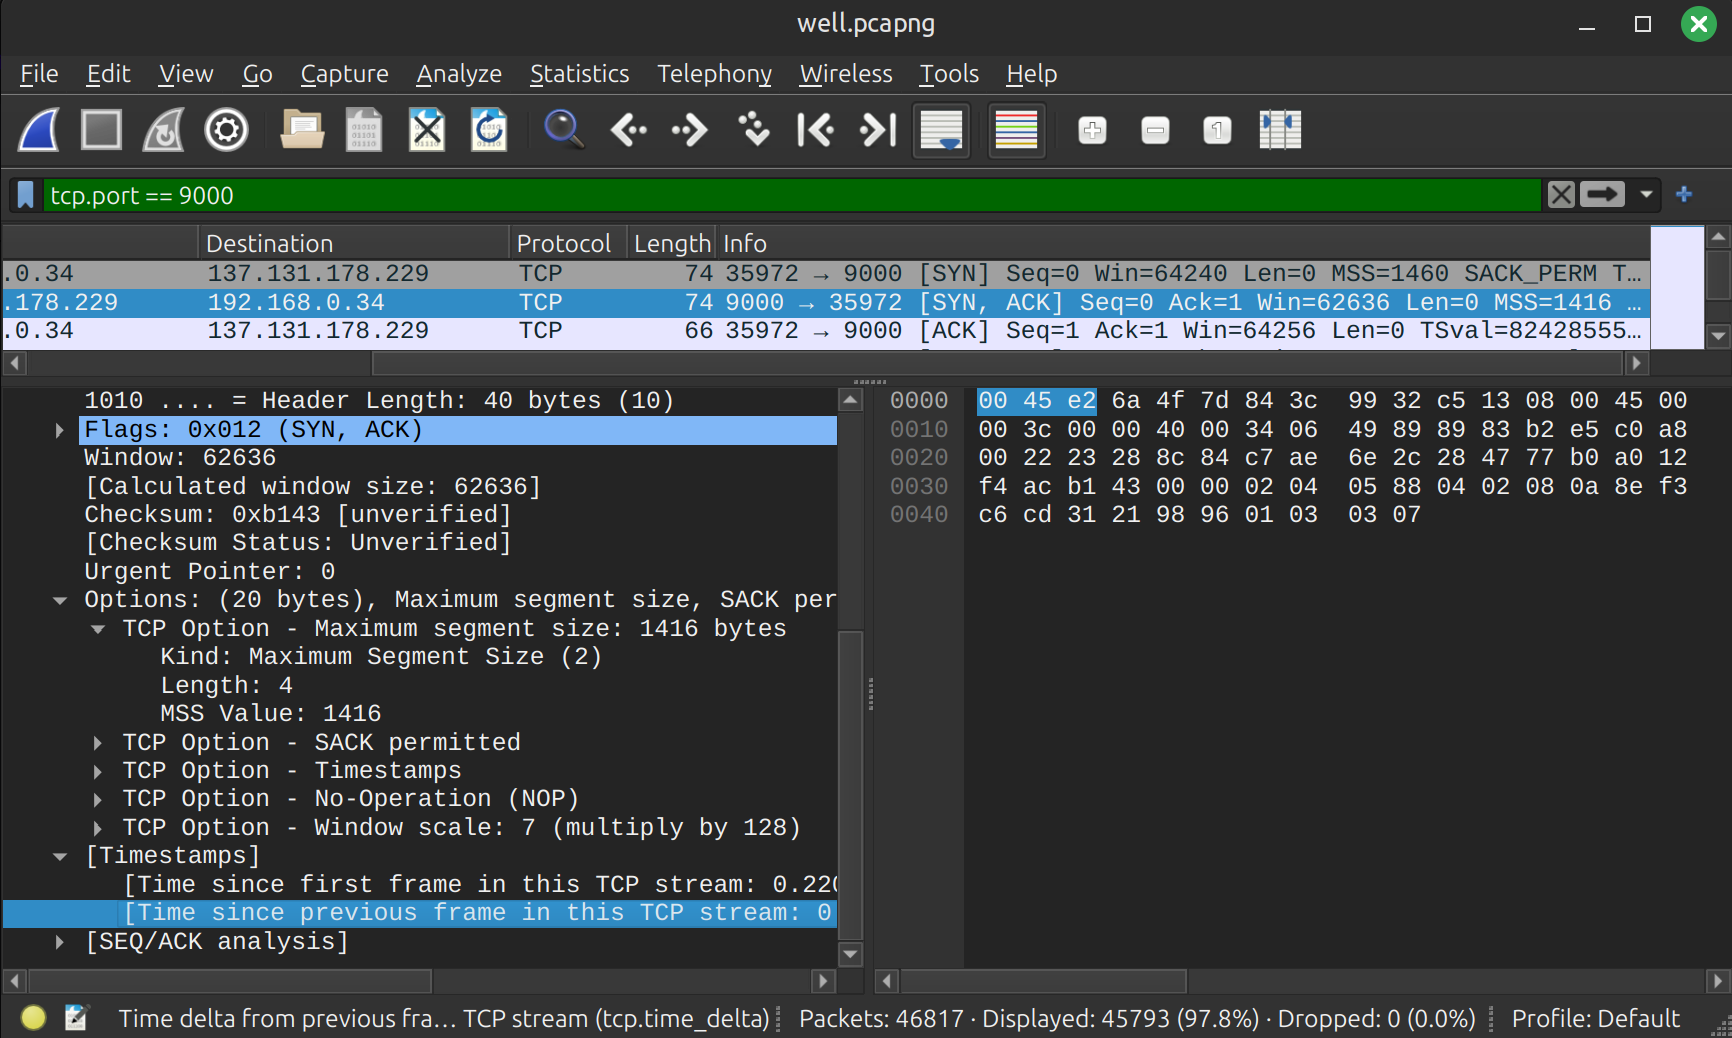
\includegraphics[width=0.8\textwidth]{figuras/q1-handshake.png}
\caption{Three-way handshake (SYN, SYN-ACK e ACK) com os campos TCP expandidos.}
\label{fig:handshake}
\end{figure}

\subsection{Questão 2}

\begin{figure}[H]
\centering
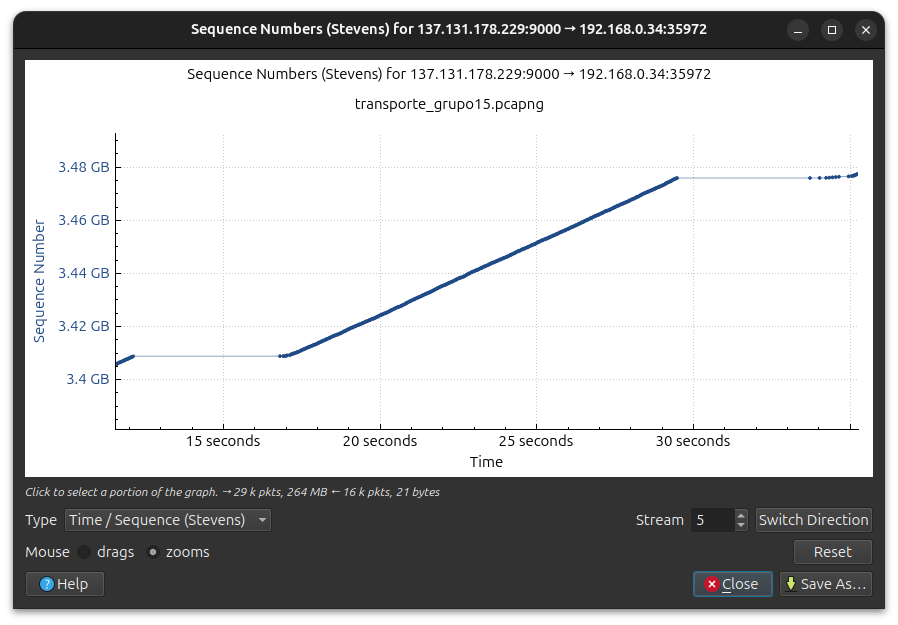
\includegraphics[width=0.8\textwidth]{figuras/Q2-graphZoom.png}
\caption{Gráfico Stevens: Número de sequência TCP vs. Tempo.}
\label{fig:StevensGraphZoom}
\end{figure}

\begin{figure}[H]
\centering
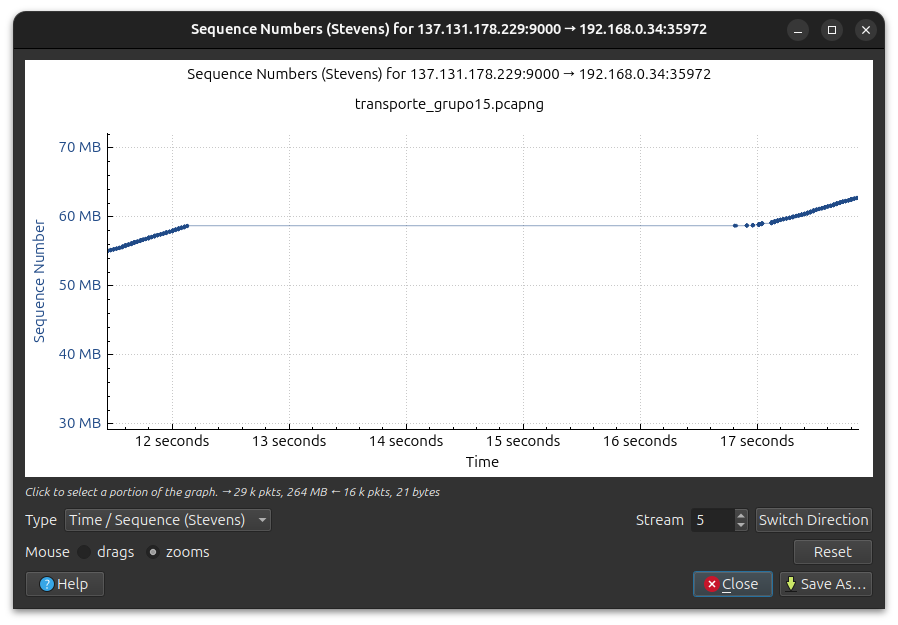
\includegraphics[width=0.8\textwidth]{figuras/PrimInterrupcao.png}
\caption{Gráfico Stevens Zoomed in para encontrar instantes de inicio da primeira interrupção mais facilmente.}
\label{fig:primeiraInterrupcao}
\end{figure}

\begin{figure}[H]
\centering
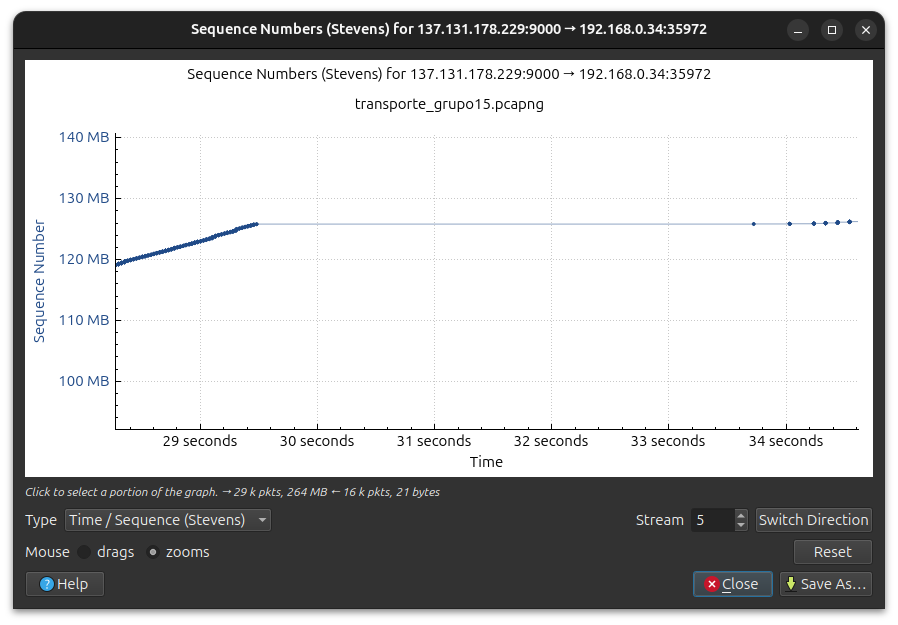
\includegraphics[width=0.8\textwidth]{figuras/SegInterrupcao.png}
\caption{Gráfico Stevens Zoomed in para encontrar instantes de inicio da segunda interrupção mais facilmente.}
\label{fig:segundaInterrupcao}
\end{figure}

\subsubsection*{(a) Instante das interrupções no fluxo de dados}
Analisando o gráfico de Stevens e as duas interrupções nítidas na transmissão de dados, observa-se que, considerando como início da interrupção o instante em que o número de bytes transferidos permanece aproximadamente constante por um determinado período, a primeira interrupção ocorre por volta de 12,12 segundos, conforme mostrado na Figura \ref{fig:primeiraInterrupcao}. Já a segunda interrupção ocorre aproximadamente em 29,48 segundos, conforme mostrado na Figura \ref{fig:segundaInterrupcao}.

\subsubsection*{(b) Bytes transferidos até as interrupções}

A partir do gráfico de Stevens, é possível estimar a quantidade de bytes transferidos até cada interrupção,
sendo até a primeira interrupção aproximadamente 58.71 MB, e até a segunda interrupção aproximadamente 125.82 MB.

\subsubsection*{(c) Quanto tempo durou as interrupções e como o inicio e o fim foram determinados}

A primeira interrupção durou até aproximadamente 16.8 segundos, sendo um total de aproximadamente 4.68 segundos.
Já a segunda interrupção durou até aproximadamente 33.72 segundos, totalizando aproximadamente 5.32 segundos. //
O início e o fim das interrupções foram determinados observando os momentos em que o número de bytes transferidos 
estabilizava por um período, indicando uma pausa na transmissão de dados.

\subsection{Questão 3}

\begin{figure}[H]
\centering
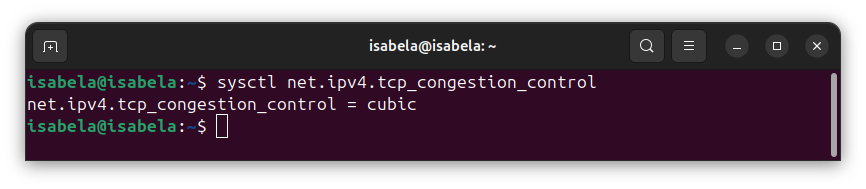
\includegraphics[width=0.8\textwidth]{figuras/TCP-terminal.png}
\caption{Identificação do algoritmo de controle de
congestionamento TCP em uso}
\label{fig:TerminalCubic}
\end{figure}

\begin{figure}[H]
\centering
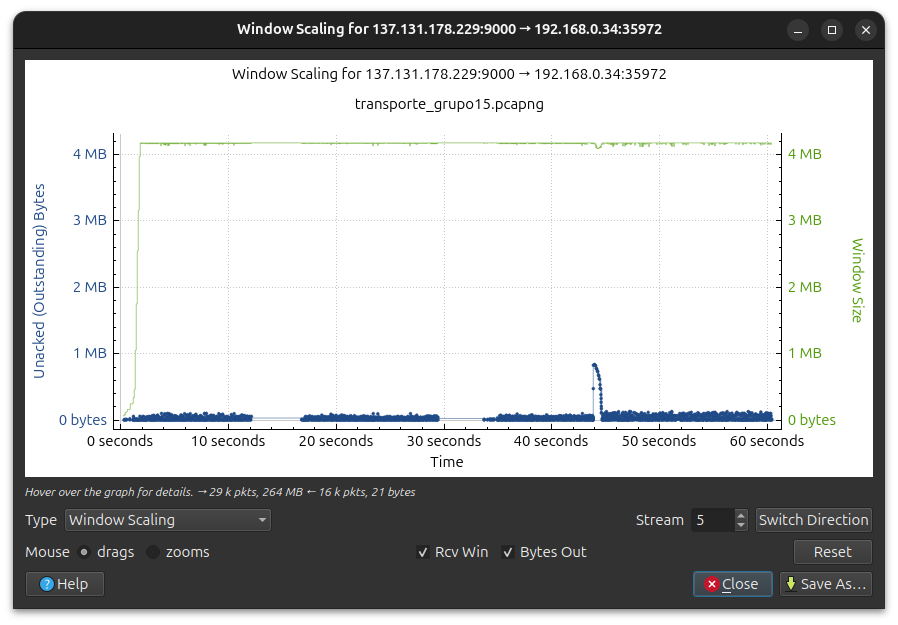
\includegraphics[width=0.8\textwidth]{figuras/rWin-bOut-graph.png}
\caption{Gráfico Window Scaling contendo as curvas Bytes Out e Rcv Win ao longo da sessão TCP.}
\label{fig:ByteOuterWin}
\end{figure}

\begin{figure}[H]
\centering
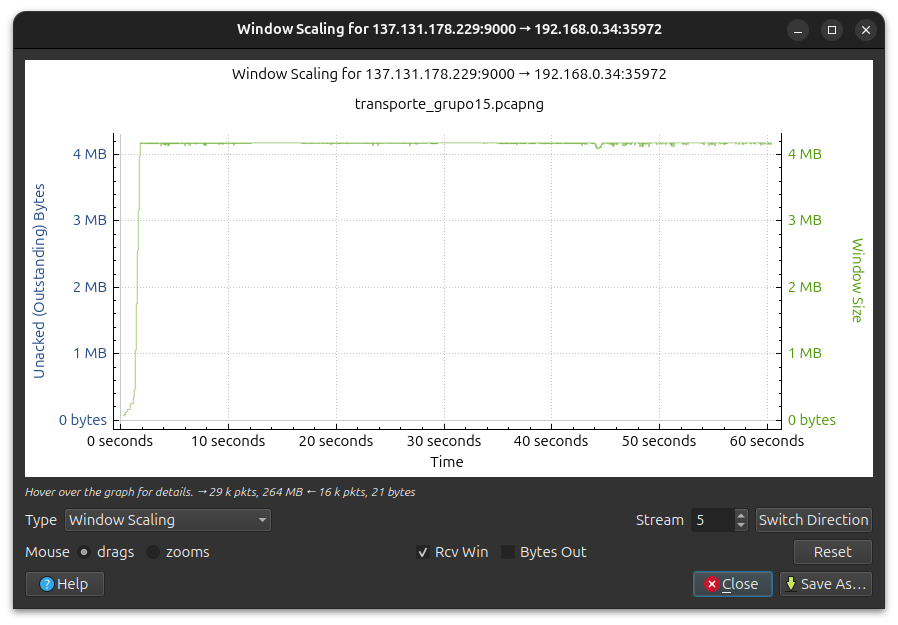
\includegraphics[width=0.8\textwidth]{figuras/rcvWin-graph.png}
\caption{Curva Rcv Win (janela de recepção anunciada pelo receptor).}
\label{fig:RcvWin}
\end{figure}

\begin{figure}[H]
\centering
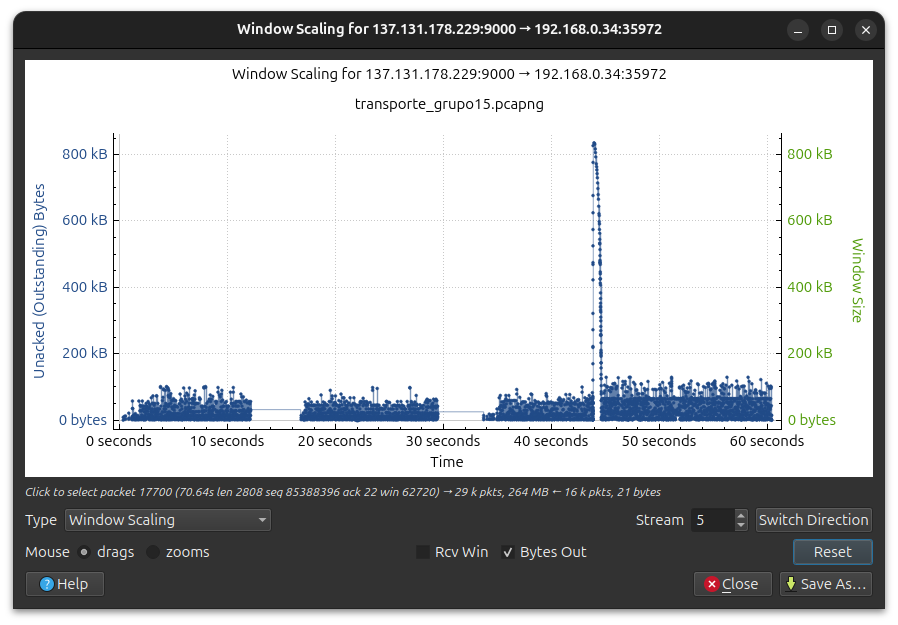
\includegraphics[width=0.8\textwidth]{figuras/bytesOut-graph.png}
\caption{Curva Bytes Out (bytes em voo durante a transferência).}
\label{fig:Bout}
\end{figure}

\subsubsection*{(a) Comportamento de Byte Out nos primeiros segundos da transferência}
Nos primeiros segundos da transferência, o gráfico de Byte Out apresenta um crescimento relativamente constante, 
diferente do esperado para um slow start, onde o número de bytes enviados dobraria a cada RTT. 


\subsubsection*{(b) Comportamento de Byte Out e rcvWin durante as interrupções}
Durante as interrupções, tanto a curva Bytes Out quanto a curva Rcv Win permaneceram 
aproximadamente constantes, indicando ausência de crescimento significativo da quantidade de dados em voo 
durante os períodos de pausa.

\subsubsection*{(c) Comportamento de Byte Out após as interrupções}
A retomada dos Byte Out foi abrupta, ele retoma os fluxo assim como estava anterior a interrupção.


\subsubsection*{(d) É consistente com Kurose para o algoritmos cubic}
Como o gráfico de Byte Out se mantem relativamente constante e baixo durante, não foi possível identificar 
claramente o comportamento cúbico esperado.

\subsection{Questão 4}

\subsubsection*{(a) Filtro tcp.analysis.duplicate_ack}

\begin{figure}[H]
\centering
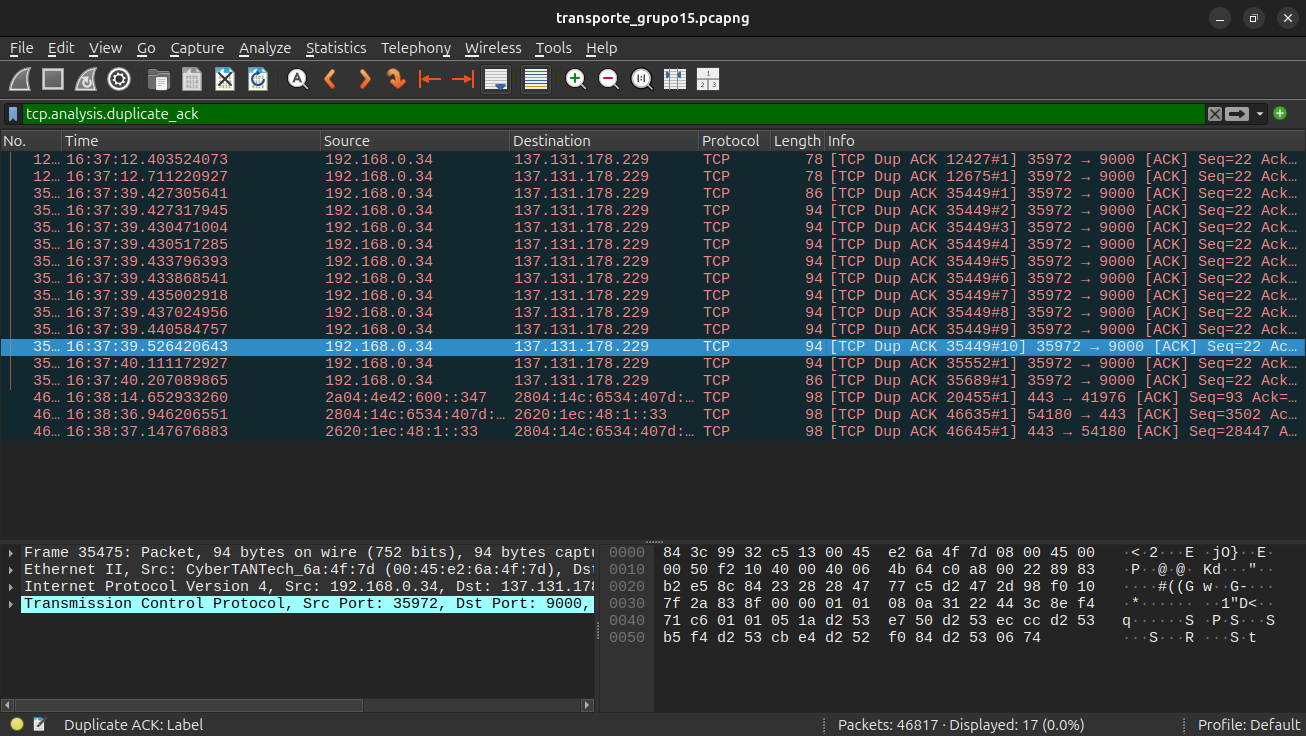
\includegraphics[width=0.8\textwidth]{figuras/filtro-dupAck.png}
\caption{Pacotes identificados pelo filtro tcp.analysis.duplicate_ack.}
\label{fig:FiltroDupAck}
\end{figure}

Aplicando o filtro \textit{tcp.analysis.duplicate_ack} no Wireshark, 
foram identificados 17 ACKs duplicados, sendo 10 a maior sequência consecutiva observada e o Acknowledgment Number 
pedido por ela 177782636.

\subsubsection*{(b) Filtro tcp.analysis.out_of_order}

\begin{figure}[H]
\centering
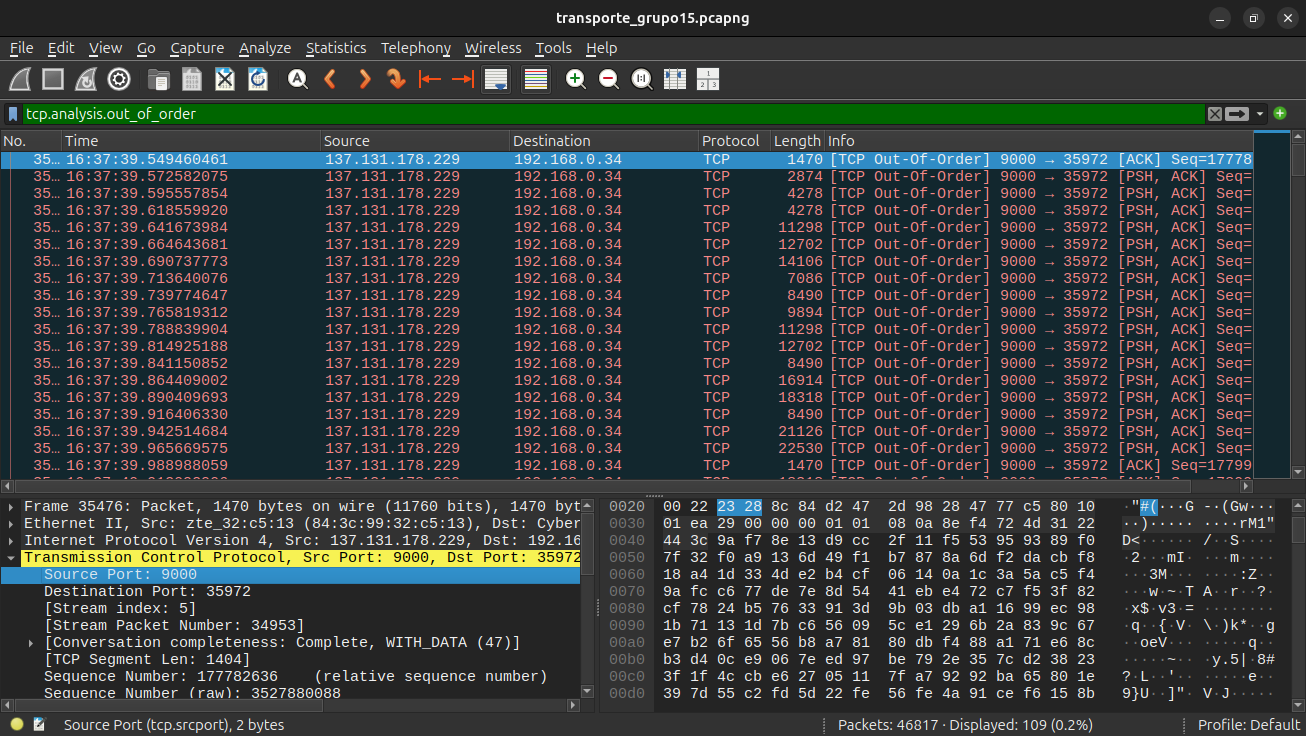
\includegraphics[width=0.8\textwidth]{figuras/filtro-outOfOrder.png}
\caption{Pacotes identificados pelo filtro tcp.analysis.out_of_order.}
\label{fig:FiltroOutOfOrder}
\end{figure}

Aplicando o filtro \textit{tcp.analysis.out_of_order} no Wireshark, 
forma detectados 109 pacotes out of order. Nesse caso, diferenciamos Out of Order de Perda real, porque 
um pacote "fora de ordem", como o nome já diz, é retransmitido pouco depois, gerando Duplicate ACKs temporários.
No entanto, Perda Real tem duplicate ACKs persistentes, seguidos de retransmissões.

\subsubsection*{(c) Filtro tcp.analysis.fast_retransmission}

\begin{figure}[H]
\centering
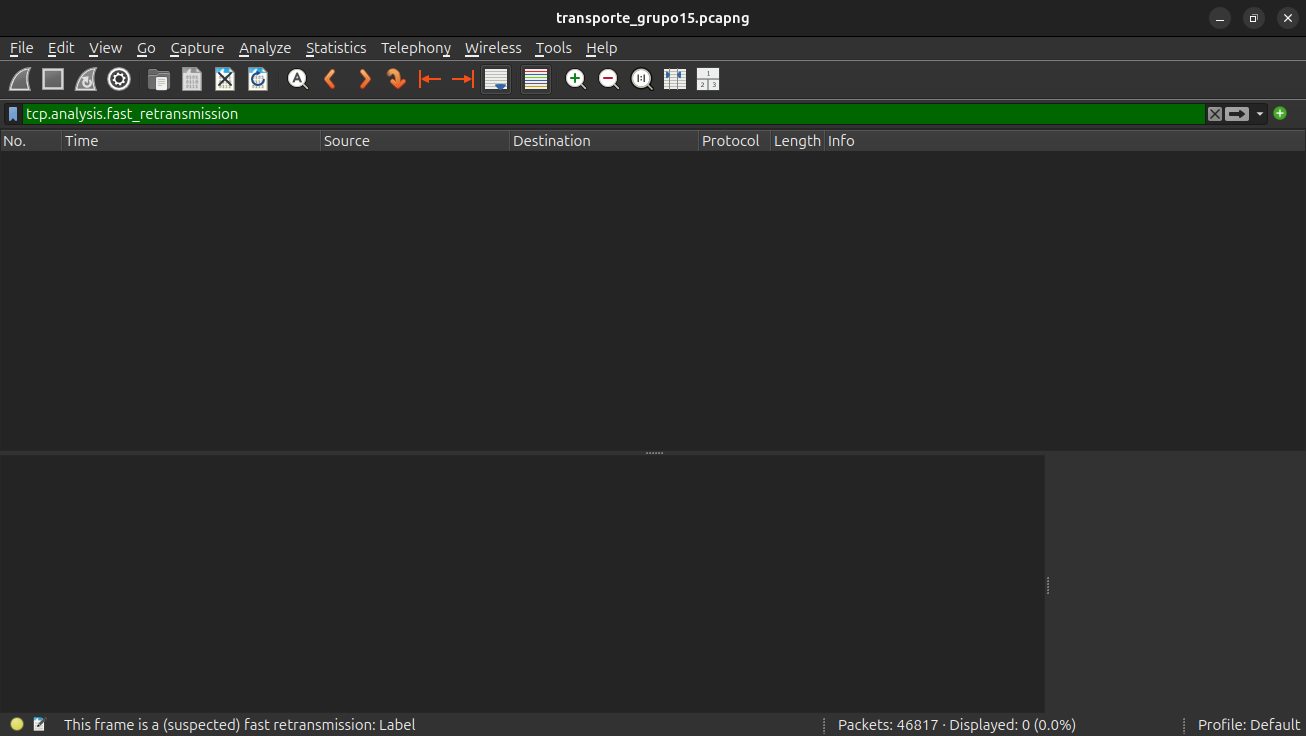
\includegraphics[width=0.8\textwidth]{figuras/filtro-fastRetransmission.png}
\caption{Resultado do filtro tcp.analysis.fast_retransmission.}
\label{fig:FiltroFastRetransmission}
\end{figure}

Não houveram retransmissões rápidas, pois o filtro \textit{tcp.analysis.fast_retransmission} 
não identificou nenhum pacote correspondente. No entanto utilizamos o filtro \textit{tcp.analysis.retransmission} 
para verificar se houve retransmissões.

\begin{figure}[H]
\centering
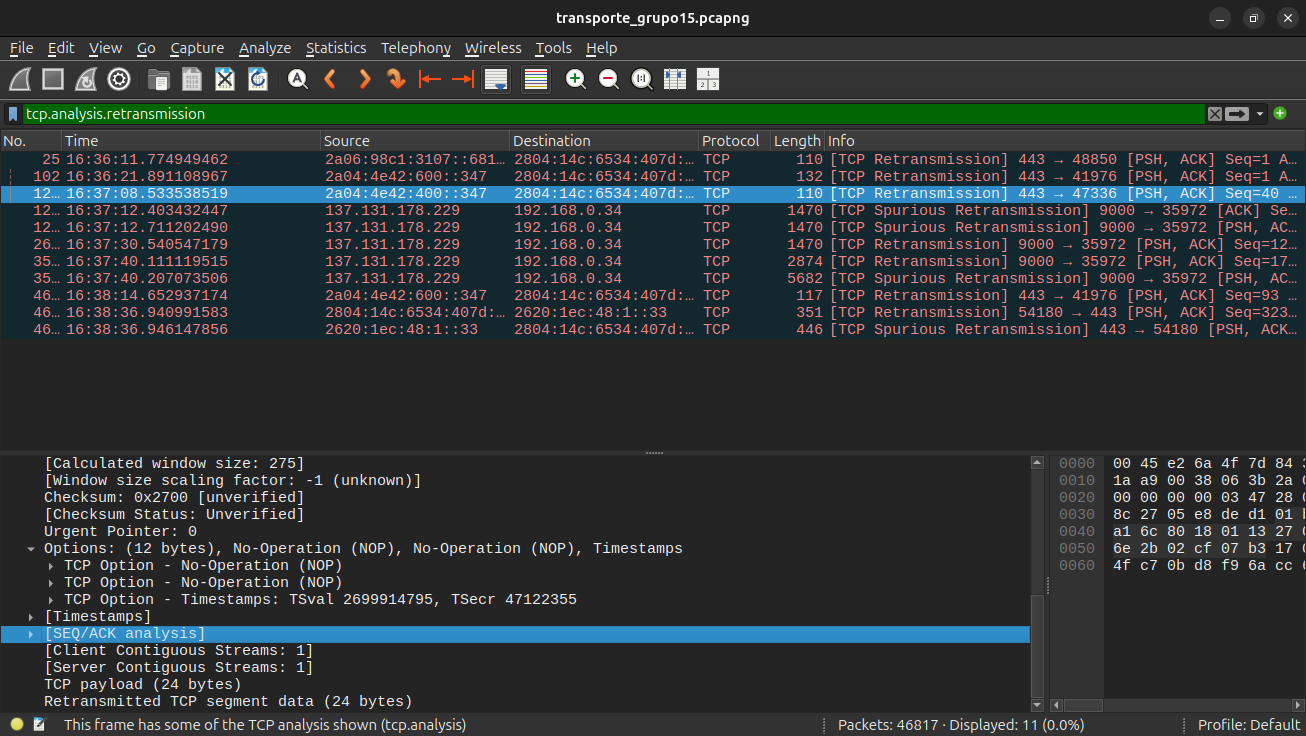
\includegraphics[width=0.8\textwidth]{figuras/filtro-retransmission.png}
\caption{Pacotes identificados pelo filtro tcp.analysis.retransmission.}
\label{fig:FiltroRetransmission}
\end{figure}


Foram identificados 11 pacotes retransmitidos, indicando que houve perda de pacotes durante a transferência.

Para conseguirmos olhar os SACK foi utilizado o filtro \textit{tcp.options.sack}.

\begin{figure}[H]
\centering
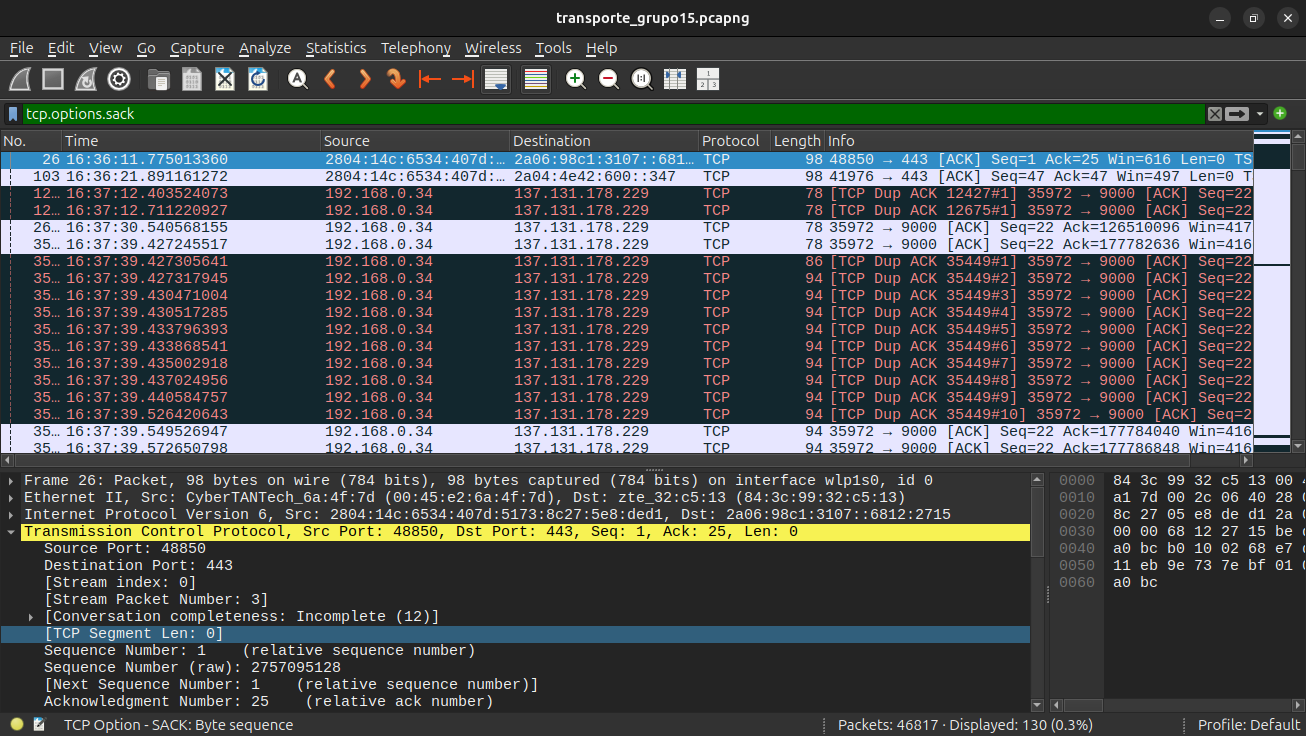
\includegraphics[width=0.8\textwidth]{figuras/filtro-optionsSack.png}
\caption{Pacotes contendo opções SACK.}
\label{fig:FiltroSack}
\end{figure}

\begin{figure}[H]
\centering
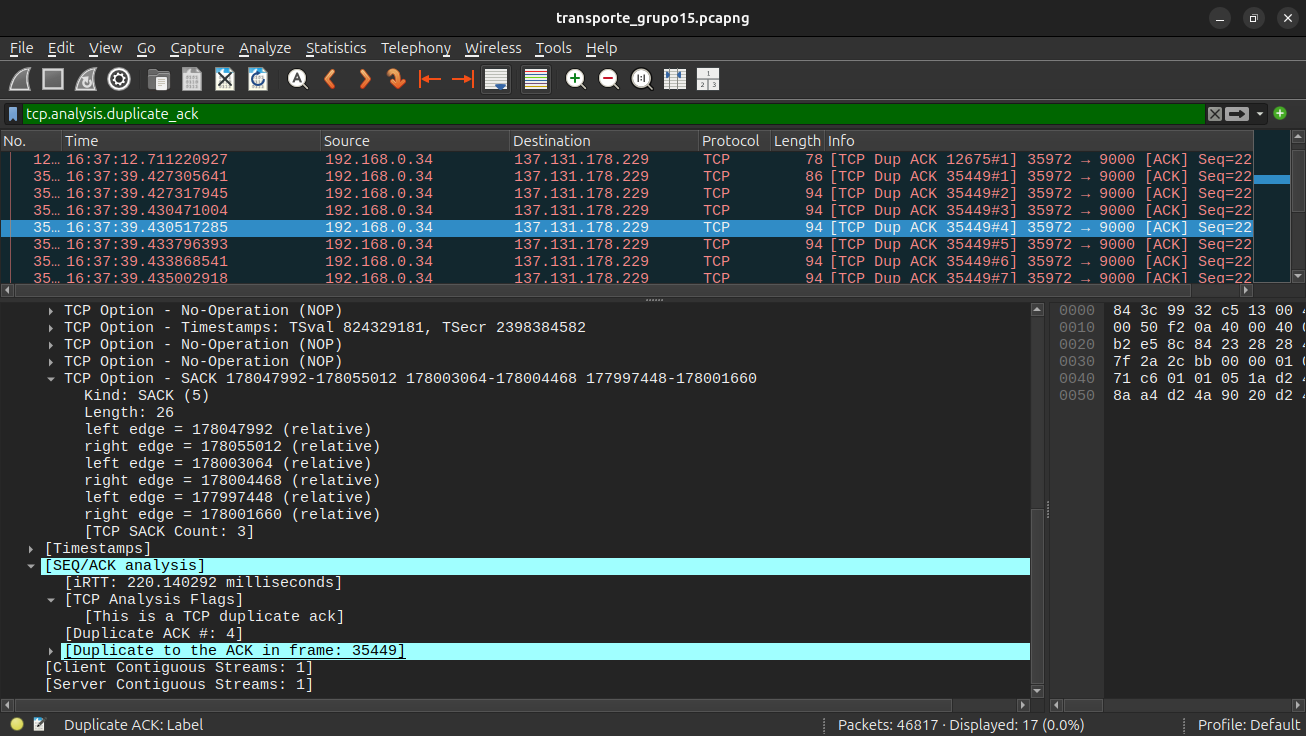
\includegraphics[width=0.8\textwidth]{figuras/campoSACK.png}
\caption{Campos SACK expandidos no painel inferior do Wireshark.}
\label{fig:CampoSack}
\end{figure}

Ao aplicar o filtro \textit{tcp.analysis.fast\_retransmission} no Wireshark, observa-se que \textbf{não ocorreu nenhuma retransmissão rápida (0 ocorrências)}, visto que o filtro não retornou nenhum pacote correspondente[cite: 26]. 

Contudo, ao analisar as retransmissões gerais capturadas pelo filtro \textit{tcp.analysis.retransmission} [cite: 27] e inspecionar os detalhes de sinalização nas figuras \ref{fig:FiltroSack} e \ref{fig:CampoSack}, respondem-se aos questionamentos sobre o frame selecionado (Frame pertencente ao instante 16:37:39, que faz parte do bloco de ACKs duplicados):

\begin{itemize}
    \item \textbf{O SACK estava habilitado?} Sim, o mecanismo SACK (\textit{Selective Acknowledgment}) estava ativo e sendo utilizado na conexão, conforme indicado pela presença da opção TCP nos cabeçalhos dos pacotes capturados[cite: 29].
    \item \textbf{Quantos blocos SACK (SACK Count) foram informados pelo receptor?} O receptor informou um \textbf{\textit{SACK Count} de 3}, ou seja, foram reportados 3 blocos seletivos distintos de dados recebidos no buffer.
    \item \textbf{O que cada bloco Left Edge / Right Edge representa?} 
    \begin{itemize}
        \item \textbf{\textit{Left Edge} (Borda Esquerda):} Representa o número de sequência inicial (o primeiro byte) de um bloco isolado de dados que o receptor já recebeu corretamente e guardou em seu buffer, sucedendo uma lacuna de dados perdidos.
        \item \textbf{\textit{Right Edge} (Borda Direita):} Representa o número de sequência imediatamente posterior ao último byte consecutivamente recebido daquele mesmo bloco (o limite superior, não inclusivo).
    \end{itemize}
    A diferença entre a \textit{Right Edge} e a \textit{Left Edge} determina o tamanho exato em bytes daquele segmento recebido fora de ordem.
\end{itemize}

\subsubsection*{(d) Natureza da retransmissão, determinação e tempo decorrido}

A retransmissão dos dados associados a esse evento \textbf{não ocorreu por Fast Retransmit convencional e nem por Timeout clássico (RTO)}, mas sim por meio de um mecanismo de \textbf{Retransmissão Rápida Orientada a SACK (\textit{SACK-based Fast Retransmission})}. 

\paragraph{Como isso foi determinado:} 
Determinamos isso a partir de duas evidências principais presentes nos logs:
\begin{enumerate}
    \item O filtro purista de \textit{Fast Retransmission} do Wireshark não acusou o frame[cite: 26], o que descarta o gatilho padrão de 3 ACKs duplicados idênticos sem opções.
    \item A análise temporal e a presença dos múltiplos ACKs duplicados (\textit{TCP Dup ACK}) no mesmo milissegundo descartam o \textit{Timeout}. Em um cenário de \textit{Timeout}, o transmissor cessaria o envio, esperaria o temporizador expirar (uma pausa longa de centenas de milissegundos) e então retransmitiria. Aqui, os dados continuaram fluindo e o receptor continuou gerando ACKs duplicados enriquecidos com mapas de SACK (informando as \textit{Edges}) para avisar precisamente quais segmentos chegaram depois da lacuna, permitindo que o transmissor fizesse a recuperação ágil sem esperar o estouro de um temporizador.
\end{enumerate}

\paragraph{Tempo decorrido entre o envio original e a retransmissão:}
Conforme explicitado pelo próprio Wireshark na análise de \textit{SEQ/ACK analysis} da flag de erro (exibida no painel inferior da Figura \ref{fig:CampoSack}), o valor medido para o tempo de ida e volta medido para esse evento de retransmissão (\textit{iRTT}) foi de \textbf{220.140292 milissegundos}. Esse tempo reflete o intervalo aproximado necessário para que o transmissor enviasse o segmento original, o receptor detectasse a falta através dos segmentos subsequentes, enviasse os ACKs duplicados com as opções SACK e o transmissor processasse e retransmitisse o pacote faltante.



\subsection{Questão 5}
\subsubsection*{(a) Throughput médio reportado pelo cliente}

Ao final da execução do cliente foi apresentado o seguinte resumo:

\begin{verbatim}
Duração         : 60.0s
Total recebido  : 193.00 MB
Throughput médio: 3.22 MB/s
\end{verbatim}

O valor reportado foi: $3.22,\text{MB/s}$. Apesar de o programa utilizar o termo \textit{Throughput médio}, o valor medido pelo cliente está mais próximo de um \textit{goodput}, pois a aplicação contabiliza apenas os dados efetivamente recebidos pela aplicação de usuário. Dessa forma, cabeçalhos TCP, IP, Ethernet e eventuais retransmissões não fazem parte da quantidade de dados considerada pelo cliente.

\subsubsection*{(b) Vazão observada no Wireshark}

A ferramenta \textit{Statistics $\rightarrow$ Conversations (TCP)} apresentou os seguintes resultados para o fluxo analisado: Pacotes totais: 45793; Bytes totais: 267 MB; Pacotes A $\rightarrow$ B: 16394; Bytes A $\rightarrow$ B: 1 MB; Pacotes B $\rightarrow$ A: 29399; Bytes B $\rightarrow$ A: 266 MB; Taxa A $\rightarrow$ B: 143 kbps; Taxa B $\rightarrow$ A: 35 Mbps.

A taxa relevante para a transferência principal é a direção servidor $\rightarrow$ cliente (B $\rightarrow$ A), cujo valor médio foi aproximadamente: $35,\text{Mbps}$. A ferramenta \textit{Conversations} contabiliza os bytes observados na captura e, portanto, inclui o overhead dos protocolos observados durante a transmissão. Já o \textit{IO Graph} exibe a evolução temporal da taxa de transmissão ao longo da sessão, permitindo visualizar oscilações e períodos de maior ou menor utilização da rede.

\subsubsection*{(c) Comparação entre os valores}

Convertendo o valor informado pelo cliente para megabits por segundo: $3.22,\text{MB/s}\times8=25.76,\text{Mbps}$. Assim, $\text{Goodput}\approx25.76,\text{Mbps}$. Enquanto isso, o Wireshark indicou aproximadamente $\text{Throughput}\approx35,\text{Mbps}$. Os valores não são iguais. O valor obtido no Wireshark é maior porque considera não apenas os dados úteis entregues à aplicação, mas também os cabeçalhos dos protocolos e outros bytes transmitidos pela conexão TCP. Portanto, $\text{Throughput}>\text{Goodput}$, o que está de acordo com o comportamento esperado para uma transferência TCP real.

\subsubsection*{(d) Cálculo do overhead esperado}

Conforme indicado no enunciado, considera-se um payload de 1390 bytes por segmento, além de 20 bytes de cabeçalho TCP e 20 bytes de cabeçalho IP. O overhead total por segmento é, portanto, de 40 bytes.

Aplicando a fórmula fornecida:

$$\text{Overhead}(\%)=\frac{\text{Cabeçalhos}}{\text{Payload}+\text{Cabeçalhos}}\times100$$

$$\text{Overhead}(\%)=\frac{40}{1390+40}\times100$$

$$\text{Overhead}(\%)=\frac{40}{1430}\times100$$

$$\text{Overhead}(\%)\approx2.80\%$$

Portanto, espera-se que aproximadamente 2,8\% da capacidade transmitida seja consumida apenas pelos cabeçalhos TCP e IP. Entretanto, a diferença observada entre o throughput medido no Wireshark ($35,\text{Mbps}$) e o goodput medido pela aplicação ($25.76,\text{Mbps}$) foi significativamente maior que 2,8\%. Isso indica que, além dos cabeçalhos TCP/IP considerados no cálculo simplificado, outros fatores contribuíram para a diferença observada, como ACKs, controle de congestionamento, pausas introduzidas pelo servidor durante o experimento e possíveis retransmissões. Dessa forma, os resultados obtidos são compatíveis com o comportamento esperado de uma conexão TCP real, mas não podem ser explicados apenas pelos 40 bytes de cabeçalhos considerados no cálculo teórico.

\subsection*{Evidências Experimentais}

\begin{figure}[H]
\centering
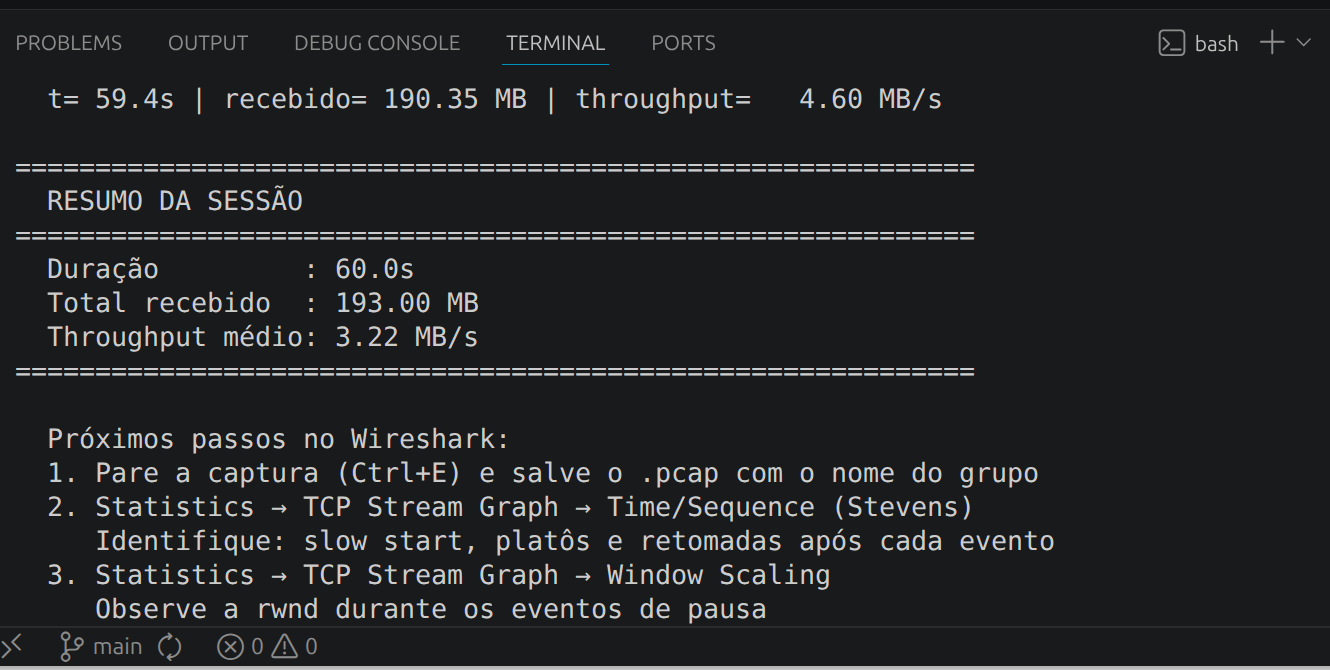
\includegraphics[width=0.85\textwidth]{figuras/q5-terminal.png}
\caption{Resumo da sessão exibido pelo cliente.}
\label{fig:q5terminal}
\end{figure}

\begin{figure}[H]
\centering
\includegraphics[width=0.85\textwidth]{figuras/q5-conversations.png}
\caption{Statistics $\rightarrow$ Conversations (TCP).}
\label{fig:q5conversations}
\end{figure}

\begin{figure}[H]
\centering
\includegraphics[width=0.85\textwidth]{figuras/q5-iograph.png}
\caption{Statistics $\rightarrow$ IO Graph com filtro tcp.stream eq 0.}
\label{fig:q5iograph}
\end{figure}

\section{Conclusão}

A captura analisada permitiu investigar diferentes mecanismos do protocolo TCP por meio de evidências obtidas no Wireshark e na aplicação cliente. Foram examinados aspectos relacionados ao estabelecimento da conexão, ao fluxo de dados, ao controle de congestionamento, às retransmissões e à vazão observada durante a transferência.

De modo geral, os resultados obtidos mostraram como conceitos teóricos da camada de transporte se manifestam em uma comunicação TCP real, evidenciando a utilidade de ferramentas de análise de tráfego para o estudo e diagnóstico de protocolos de rede.

\begin{thebibliography}{9}

\bibitem{tanenbaum}
TANENBAUM, Andrew S.;
WETHERALL, David J.
\textit{Redes de Computadores}.
5. ed.
São Paulo: Pearson, 2011.

\end{thebibliography}

\end{document}
